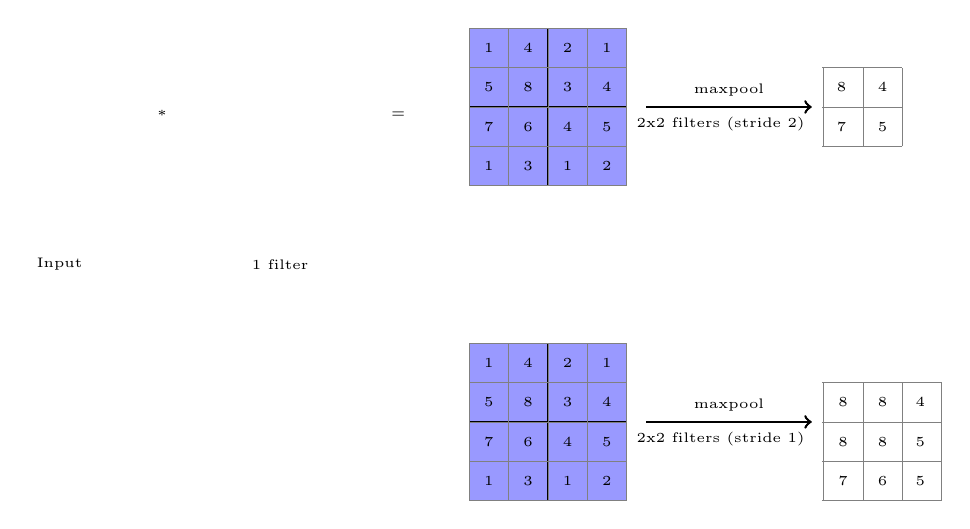
\begin{tikzpicture}
	\onslide<1->{   \renewcommand{\forefillColor}{black!50!white}
		\renewcommand{\borderColor}{white}
		\renewcommand{\toprsidefillcolor}{black!50!white!50}
		\handmadecube{0.5}{2.0}{0.7}{0}{0}
		\node(A) at (-0.2,-2.5){\tiny{Input}};}
  
	\onslide<2->{   \node(star) at (1.1,-0.6){\tiny{*}};
   
		%% filter
		\renewcommand{\forefillColor}{purple!50!white}
		\renewcommand{\borderColor}{white}
		\renewcommand{\toprsidefillcolor}{purple!50!white!50}
		\handmadecube{1.7}{2.3}{0.04}{3.5}{0.5}
		\node(A) at (2.6,-2.5){\tiny{1 filter}};
	}
  
	%%
	\onslide<3->{\node(star) at (4.1,-0.6){\tiny{=}};}
	%%
	\onslide<7>{    \filldraw[fill=blue!40!white, draw=black] (4.99999,-1.5+2) rectangle (4.99999+1,-1.5+2-1);}
  
	\onslide<8>{\filldraw[fill=blue!40!white, draw=black] (4.99999+1,-1.5+2) rectangle (4.99999+1+1,-1.5+2-1);}
  
	\onslide<9>{\filldraw[fill=blue!40!white, draw=black] (4.99999,-1.5+1) rectangle (4.99999+1,-1.5);}
  
	\onslide<10>{\filldraw[fill=blue!40!white, draw=black] (4.99999+1,-1.5+1) rectangle (4.99999+1+1,-1.5);}
	\onslide<3->{   \draw[step=0.5cm,gray,very thin] (4.99999,-1.5) grid (7,0.5);}
	%%
	
  
	\onslide<4->{   \node(A) at (5.25,0.25){\tiny{1}};
	\node(A) at (5.75,0.25){\tiny{4}};
	\node(A) at (6.25,0.25){\tiny{2}};
	\node(A) at (6.75,0.25){\tiny{1}};

	\node(A) at (5.25,-0.25){\tiny{5}};
	\node(A) at (5.75,-0.25){\tiny{8}};
	\node(A) at (6.25,-0.25){\tiny{3}};
	\node(A) at (6.75,-0.25){\tiny{4}};

	\node(A) at (5.25,-0.75){\tiny{7}};
	\node(A) at (5.75,-0.75){\tiny{6}};
	\node(A) at (6.25,-0.75){\tiny{4}};
	\node(A) at (6.75,-0.75){\tiny{5}}; 

	\node(A) at (5.25,-1.25){\tiny{1}};
	\node(A) at (5.75,-1.25){\tiny{3}};
	\node(A) at (6.25,-1.25){\tiny{1}};
	\node(A) at (6.75,-1.25){\tiny{2}};}      
	%%
	\onslide<5->{\draw[->,thick] (5.75+1.5,-0.5) -- (5.75+3.6,-0.5) node [pos=0.5,above] {\text{\tiny{maxpool}}};
		\draw[->,thick]  (5.75+1.5,-0.5) -- (5.75+3.6,-0.5) node [pos=0.45,below] {\tiny{2x2 filters (stride 2)}}; }
  
  
	\onslide<6->{   \draw[step=0.5cm,gray,very thin] (9.48559,-1) grid (10.5,0);}
	%%
	\onslide<7->{   \node(A) at (9.73,-0.25){\tiny{8}};    }
	\onslide<8->{   \node(A) at (10.25,-0.25){\tiny{4}};    }
  
	\onslide<9->{   \node(A) at (9.73,-0.75){\tiny{7}};    }
	\onslide<10->{  \node(A) at (10.25,-0.75){\tiny{5}};    }
	%%
	\onslide<14>{   \filldraw[fill=blue!40!white, draw=black] (4.99999,-5.5+2) rectangle (4.99999+1,-5.5+2-1);}
  
	\onslide<15>{   \filldraw[fill=blue!40!white, draw=black] (4.99999+0.5,-5.5+2) rectangle (4.99999+1.5,-5.5+2-1);}
  
	\onslide<17>{   \filldraw[fill=blue!40!white, draw=black] (4.99999,-5.5+2-0.5) rectangle (4.99999+1,-5.5+2-1.5);}
  
	\onslide<18>{   \filldraw[fill=blue!40!white, draw=black] (4.99999+0.5,-5.5+2-0.5) rectangle (4.99999+1.5,-5.5+2-1.5);}
      
	\onslide<19>{   \filldraw[fill=blue!40!white, draw=black] (4.99999+1,-5.5+2-0.5) rectangle (4.99999+2,-5.5+2-1.5);}
  
	\onslide<16>{   \filldraw[fill=blue!40!white, draw=black] (4.99999+1,-5.5+2) rectangle (4.99999+1+1,-5.5+2-1);}
  
	\onslide<20>{   \filldraw[fill=blue!40!white, draw=black] (4.99999,-5.5+1) rectangle (4.99999+1,-5.5);}
  
	\onslide<21>{   \filldraw[fill=blue!40!white, draw=black] (4.99999+0.5,-5.5+2-1) rectangle (4.99999+1.5,-5.5);}
  
	\onslide<22>{   \filldraw[fill=blue!40!white, draw=black] (4.99999+1,-5.5+1) rectangle (4.99999+1+1,-5.5);}
  
	
	\onslide<11->{  \draw[step=0.5cm,gray,very thin] (4.99999,-5.5) grid (7,-3.5);
		%%
		\node(A) at (5.25,-3.75){\tiny{1}};
		\node(A) at (5.75,-3.75){\tiny{4}};
		\node(A) at (6.25,-3.75){\tiny{2}};
		\node(A) at (6.75,-3.75){\tiny{1}};
   
		\node(A) at (5.25,-4.25){\tiny{5}};
		\node(A) at (5.75,-4.25){\tiny{8}};
		\node(A) at (6.25,-4.25){\tiny{3}};
		\node(A) at (6.75,-4.25){\tiny{4}};
   
		\node(A) at (5.25,-4.75){\tiny{7}};
		\node(A) at (5.75,-4.75){\tiny{6}};
		\node(A) at (6.25,-4.75){\tiny{4}};
		\node(A) at (6.75,-4.75){\tiny{5}}; 
   
		\node(A) at (5.25,-5.25){\tiny{1}};
		\node(A) at (5.75,-5.25){\tiny{3}};
		\node(A) at (6.25,-5.25){\tiny{1}};
		\node(A) at (6.75,-5.25){\tiny{2}};       
		%%
	}
  
	\onslide<12->{\draw[->,thick] (5.75+1.5,-0.5-4) -- (5.75+3.6,-0.5-4) node [pos=0.5,above] {\text{\tiny{maxpool}}};
		\draw[->,thick]  (5.75+1.5,-0.5-4) -- (5.75+3.6,-0.5-4) node [pos=0.45,below] {\tiny{2x2 filters (stride 1)}};}
      
      
	\onslide<13->{  \draw[step=0.5cm,gray,very thin] (9.48,-5.5) grid (11,-4);}
	%%
	\onslide<14->{  \node(A) at (9.75,-4.25){\tiny{8}};}
	\onslide<15->{  \node(A) at (10.25,-4.25){\tiny{8}};}
	\onslide<16->{  \node(A) at (10.73,-4.25){\tiny{4}};}
  
	\onslide<17->{  \node(A) at (9.75,-4.75){\tiny{8}};}
	\onslide<18->{  \node(A) at (10.25,-4.75){\tiny{8}};}
	\onslide<19->{  \node(A) at (10.73,-4.75){\tiny{5}};}
  
	\onslide<20->{  \node(A) at (9.75,-5.25){\tiny{7}};}
	\onslide<21->{  \node(A) at (10.25,-5.25){\tiny{6}};}
	\onslide<22->{  \node(A) at (10.73,-5.25){\tiny{5}};}

\end{tikzpicture}